% ***********************************************************************************
% Pure LaTeX part to be inserted in a document (be careful of depencies of packages & commands)
% Prepared by XXX and YYY under the supervision of Arnaud de La Fortelle
% Fall 2017
% 1D heat diffusion subsection of the simulation part
% ***********************************************************************************

\subgroup{1}{Lin Yang and Bradley Cage}

\paragraph{Model presentation}

\begin{figure}[htb]
	\centering
	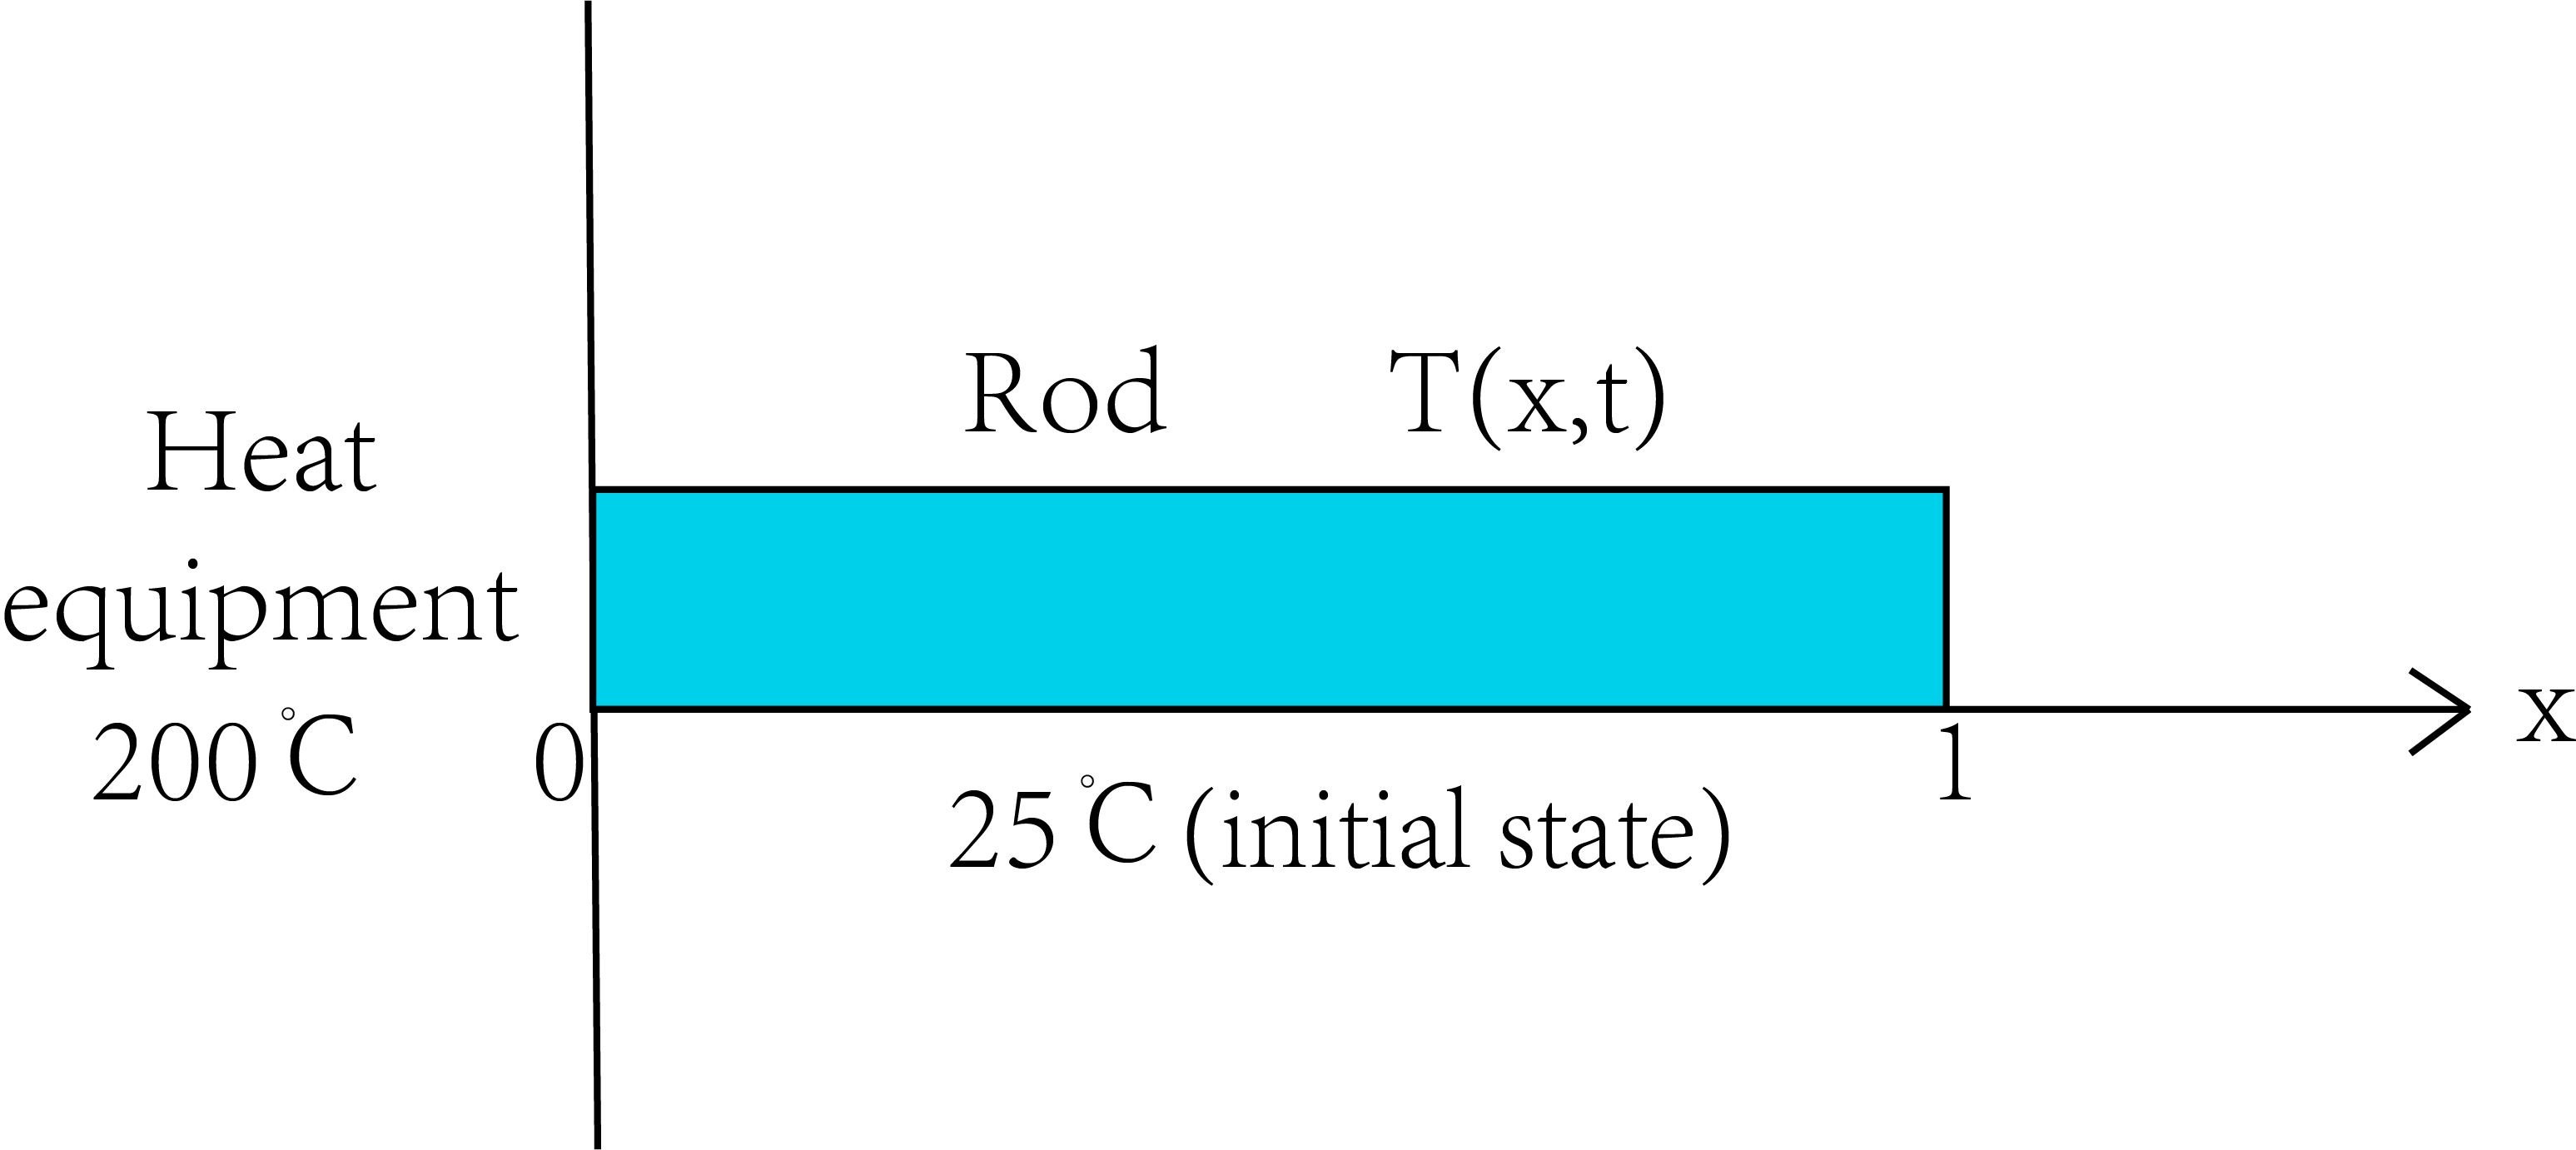
\includegraphics[width=8cm]{Figures/Heat1D_model.png}       
	\caption{The heated rod system, with the temperature at any point given by $u(x,t)$ }
	\label{fig:toto}
\end{figure}

Our system is comprised of a rod fixed to a heated wall kept at constant temperature. The length of the rod is arbitrarily taken as 1m. The initial temperature of the rod is in equilibrium with the ambient temperature at 25$^{\circ} $C and the temperature of the wall is 200$^{\circ} $C.  We represent temperature at a point on the rod at some time with the function $u(x,t)$. Note that the rod is thin with respect to its length, thus is modeled as a 1D system, that is, temperature is solely a function of rod position and time. The goal of this simulation is to show the variations in temperature of various points on the rod over time. //

We take our initial state as:
\begin{itemize}
	\item $T(0,t)=200 ^{\circ}$C
    \item $T(x,t)=25 ^{\circ}$C, $x\ne 0$
\end{itemize}

\noindent The partial differential equation of the 1D heat propagation:
\begin{equation}
 \frac{\partial u}{\partial t} = \alpha \frac{\partial^2 u}{\partial x^2}
\end{equation}
\noindent We explicitly state that $u(\dot)$ is a function of $x$ and $t$
\begin{equation}
 \frac{\partial} {\partial t}u(x,t) = \alpha \frac{\partial^2}{\partial x^2}u(x,t)
\end{equation}
\noindent We use a finite difference approximation to get compute the derivatives in space and time
\begin{equation}
\frac{u_{i}^{N+1}-u_{i}^{N}}{\Delta t} =\alpha\frac{u_{i+1}^{N}-2u_{i}^{N}+u_{i-1}^{N}}{\Delta x^2}
\end{equation}

\noindent Rearranging we reach the final form we need for our Forward Euler approximation. Note that the quantity $\alpha\frac{\Delta t}{\Delta x^2}$ is Fourier's number, with $\alpha$ being the thermal diffusivity of a material. In the following simulations, we arbitrarily choose Aluminium with $\alpha = 9.7e-5$.

\begin{equation}
u_{i}^{N+1}=u_{i}^{N}+\alpha\frac{\Delta t}{\Delta x^2}\big[ {u_{i+1}^{N}-2u_{i}^{N}+u_{i-1}^{N}}\big]
\end{equation}

\paragraph{Implementation}
We provide an implementation in Matlab. 

\begin{lstlisting}[language=Matlab, caption=Forward Euler and Plotting in MATLAB]
  % Values arbitrarily chosen. It's a useful exercise to vary these and look at the results
  T_final = 300;
  N_t = 2000;
  X_final = 1;
  N_x = 100;
  
  % Calculate time and x steps based on sampling size and # of samples
  T = linspace(0, T_final, N_t+1);
  X = linspace(0, X_final, N_x+1);
  dt = T(2) - T(1);  % Calculate delta t
  dx = X(2) - X(1);  % Calculate delta x

  alpha = 9.7e-5; % Thermal diffusivity of Aluminium in m^2/s
  Fo = (alpha*dt)/(dx^2); % Fouriers number = diffusive transport rate/storage rate
 
  % Define your initial condition here. This could be some function IC(x),
  %  however for simplicity's sake we take a rod with a uniform temperature
  %  and in contact with a hot plate at one end
  wall_temp = 200;
  init_temp = 25;
  
  % Initialize the N state and the N-1 state
  u_old = zeros(1, N_x+1); 
  u_old(:) = init_temp;
  u_old(1) = wall_temp;
  u_cur = u_old;
  u_plot = u_old;

  for t = 1:N_t
     for i = 2:N_x
     	 % Forward Euler solution to heat equation
         u_cur(i) = Fo*(u_old(i+1) - 2*u_old(i) + u_old(i-1)) + u_old(i);
     end
     u_cur(1) = wall_temp; % Set the left boundary to be our high of 200 
     u_old(:) = u_cur; % We move to the next time step, reset N-1 state
     u_plot = [u_plot; u_cur];
  end

  [X_plot,T_plot] = meshgrid(X,T); % Create 2D meshgrid to create surface plot

  surf(X_plot,T_plot,u_plot,'EdgeColor','none') % Create surface plot
  c = colorbar; % Attach colour bar and create scale
  c.Label.String = 'Temperature [C]';

  xlim([0 1]) % Add axis limits
  xlabel('Distance along rod [m]'); % Add descriptive axis labels
  ylabel('Time [s]');
  zlabel('Temperature [C]')

\end{lstlisting}


 \paragraph{Results}
\noindent We can create plots of the rods temperature as a function of time and position. This gives us insight into how the system evolves as we maintain our constant temperature. 
\begin{figure}[htb]
	\centering
	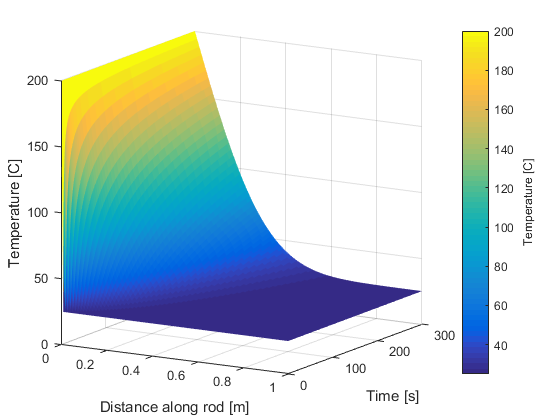
\includegraphics[width=10cm]{Figures/Heat1D_1m.png}       
	\caption{Temperature variation for the whole rod over 300 seconds}
	\label{fig:toto}
\end{figure}

\begin{figure}[htb]

	\centering
	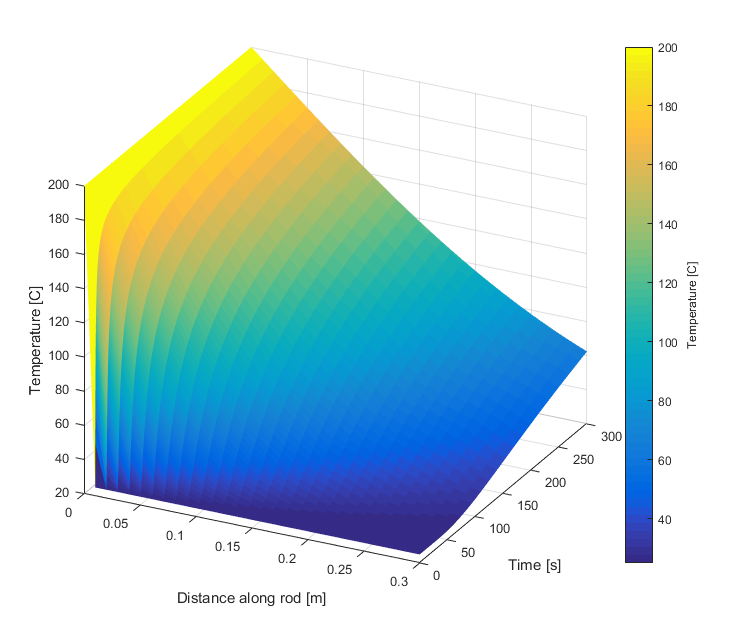
\includegraphics[width=9cm]{Figures/Heat1D_0_3m.png}       
	\caption{Temperature variation for the rod segment with x varies from 0 to 0.3m over 300 seconds}
	\label{fig:toto}
\end{figure}
\clearpage
\begin{figure}[!htb]
	\centering
	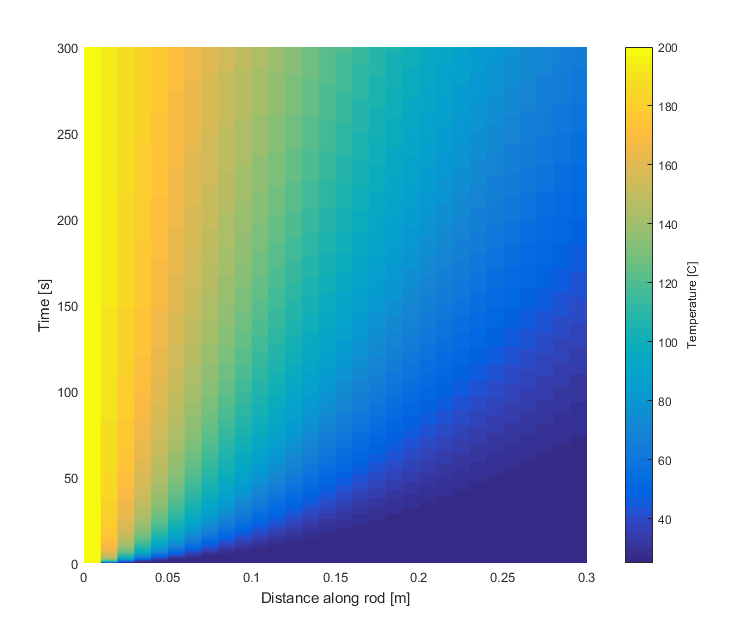
\includegraphics[width=9cm]{Figures/Heat1DTop.png}       
	\caption{Top view of the temperature variation for the whole rod over 300 seconds}
	\label{fig:toto}
\end{figure}
 
\paragraph{Interpretation}
The results we obtain are consistent with our model and the physical characteristics. We can see that from the visualization the temperature falls off as $\frac{1}{x^2}$, which is 
consitent with the theoretical definition of the Fourier number as described above. We can see pathlines of the heat front evolve quadratically over time, especially when looking 
at the system from above. 

 \paragraph{Conclusion}
Here we have learned that in examining systems such as the heated rod, we can safely analyze it as a 1D system. We were able to discretize the partial differential equations and 
apply a forward Euler simluation to yield phyiscally relevant and meaningful simulations. Through the Matlab visualization, we gain a better understanding of how heat is moving 
through the rod and the system. From the resources and analysis provided, it is trivial to create other iinitial/boundary conditions and repeat the simulations to garner a deeper
insight into the heat behaviour. This is left as an exercise to the reader. 
 
